\begin{enumerate}[label=\thesection.\arabic*.,ref=\thesection.\theenumi]
\numberwithin{equation}{enumi}

\item Why do we use compensators. \\
\solution In order to obtain the desired performance of the system, we use compensating networks.

\item What is the use of a Phase lead compensator. \\
\solution Phase lead compensator is used to increase the stability or speed of response of a system.

\item What is the use of phase lag compensator. \\
\solution Phase lag compensator lag compensator is used to reduce (but not eliminate) the steady-state error.

\item Write the general expression for the transfer function of a phase lead compensator. \\
\solution 
\begin{align}
    H(s) = \frac{(1+ \alpha s T)}{(1+T s)}
\end{align}
$\alpha$ is generally less than 1 for Phase lead compensator.

\item Find the frequency range in which phase introduced by the phase lead compensator reaches maximum \\
\solution  Transfer function can be rewritten as 
\begin{align}
    H(j\omega) = \frac{(1+ j \alpha \omega T)}{(1+j \omega T)}
\end{align}
Then phase introduced by transfer function is given by 
\begin{align}
    \phi = tan^{-1}(\alpha \omega T) - tan^{-1}(\omega T)
\end{align}
Upon differentiating
\begin{align}
    \frac{d\phi}{d\omega} = \frac{\alpha T}{1 + (\alpha \omega T)^2} - \frac{T}{1 + (\omega T)^2}
\end{align}
Equating it to zero to find the maximum
\begin{align}
    \frac{\alpha T}{1 + (\alpha \omega T)^2} = \frac{T}{1 + (\omega T)^2} \\
    \alpha(1 +(\omega T)^2) = 1 + (\omega \alpha T)^2 \\
    \alpha + \alpha(\omega T)^2 = 1 + (\omega \alpha T)^2 \\
    (\alpha - 1) = (\omega T)^2 \alpha(\alpha -1) \\
    (\omega)^2 = \frac{1}{(T^2) \alpha} \\ 
    \omega = \frac{1}{T \sqrt{\alpha}}
\end{align}
Clearly
\begin{align}
    \frac{1}{\alpha T} < \frac{1}{T \sqrt{\alpha}} < \frac{1}{T}
\end{align}
So the frequency range in which phase lead introduced by this compensator reaches maximum in 
\begin{align}
    \omega \epsilon (\frac{1}{\alpha T} , \frac{1}{T})    
\end{align}


\item Write the general expression for the transfer function of phase lag compensator. \\
\solution 
\begin{align}
    H(s) = \frac{1}{\beta}\frac{(1+ \beta s T)}{(1+T s)}
\end{align} 
$\beta$ is generally greater than 1 for Phase lead compensator.


\item
Write the general expression for the transfer function of a Phase lag-lead compensator. \\
\solution
The Transfer Function of the Phase lag-lead compensator is
\begin{align}
    H(s) = \frac{(1+ \alpha s T_1)(1+ \beta s T_2)}{(1+T_1 s)(1 + T_2 s)}
\end{align}
$\alpha$ and $\beta$ are generally chosen in such a way that
\begin{align}
    \alpha \beta = 1
\end{align}

It is to be noted that phase introduced by lag part is close to zero in the frequency range where lead part reaches maximum and vice versa.

\item Write the expression for phase introduced by phase lag-lead compensator. \\
\solution 
\begin{align}
    \phi = tan^{-1}(\frac{\omega T_1}{\beta}) + tan^{-1}( \beta \omega T_2) - tan^{-1}(\omega T_1) - tan^{-1}(\omega T_2)
\end{align}

\item Consider the Transfer function of a phase lag-lead compensator
\begin{align}
    C(s) = \frac{(1+\frac{s}{0.1})(1+\frac{s}{100})}{(1+\frac{s}{1})(1+\frac{s}{10})}
\end{align}
Find the frequency range in which the phase (lead) introduced by the compensator reaches the maximum \\ 
\solution 
Comparing the given Transfer function with with equation(1.7.1), we get $\alpha$ = 10, $T_1$ = 1, $\beta$ = 0.1, $T_2$ = 0.1.
Substituting these values in equation (1.8.1)
\begin{align}
    \phi = tan^{-1}(10\omega) + tan^{-1}(0.01\omega) - tan^{-1}(\omega) - tan^{-1}(0.1\omega)
\end{align}
As we are trying to find the range of frequencies in which Phase lead introduced by the compensator is maximum, the phase introduced by the lag part of compensator will be close to zero.
\begin{align}
    \phi = tan^{-1}(10 \omega ) - tan^{-1}(\omega )
\end{align}
This is similar to equation 1.5.2 and we already know that in this case $\phi$ is maximum for 
\begin{align}
    \omega \epsilon (0.1,1)
\end{align}

\item Verify using a python plot \\ 
\solution
\begin{lstlisting}
codes/EE18BTECH11044.py
\end{lstlisting}

\begin{figure}[h!]
\centering
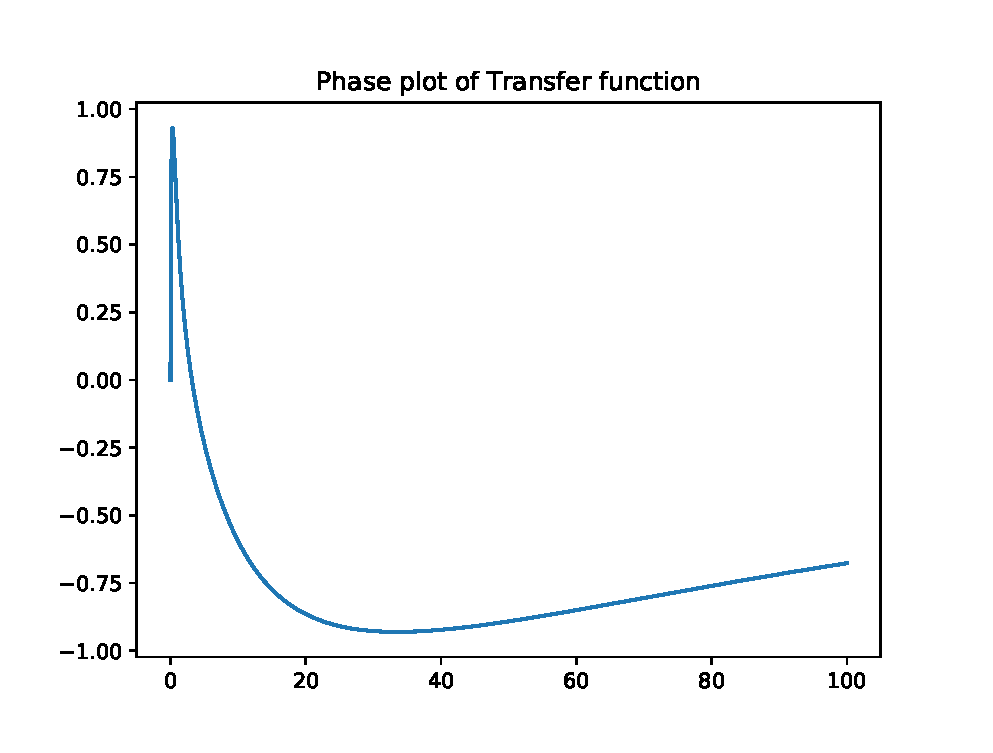
\includegraphics[width=\columnwidth]{figs/EE18BTECH11044.eps}
\end{figure}


\end{enumerate}
